\chapter{Destructive 3D phenotyping pipeline for harvestable organs}

\section{Introduction}

% Cosmetic standards (e.g., size, shape, and aesthetics) play an important role in vegetable quality standards in Northern Hemisphere countries \citep{porter_avoidable_2018}. Vegetables that do not meet this standard cannot be easily sold and are not harvested \citep{garrone_opening_2014}, which causes an unavoidable component of food loss in modern society \citep{parfitt_food_2010,teuber_food_2016}. 

Broccoli (\textit{Brassica oleracea} L.) heads are an important component of the global vegetable market. However, a certain amount of non-standardly harvested heads are wasted owing to uneven individual growth rates and the failure to meet cosmetic standards such as size, shape, and aesthetics. Traditional manual judgments for the size and quality of broccoli heads are time-consuming, laborious, and often inaccurate. Hence, there is a need to develop novel methods to quantify specific traits and accelerate the evaluation process.

Several authors have developed 2D image-based phenotyping methods for the above purpose, which are more efficient, non-destructive, and have higher throughput \citep{yang_greenness_2015,guo_easypcc_2017,zou_broccoli_2019}. However, these approaches are unable to describe the plant 3D structure due to occlusion and dimension loss when projecting onto the 2D plane. As a result, it produces inaccuracies and uncertainties for advanced phenotyping applications.

To overcome the drawbacks of 2D image-based phenotyping, several studies have paid attention to 3D approaches. \citet{paulus_measuring_2019} and \citet{kochi_introduction_2021} have summarized the current approaches to obtain 3D plant models; and a large number of studies have chosen 3D reconstruction by photogrammetry using common \gls{rgb} cameras due to the low device cost \citep{xiao_estimating_2021,zermas_3d_2020,zhang_estimating_2016}. The 3D model of an object can be calculated from images from different perspectives (view angles) with enough overlap (Fig.~\ref{fig:des1}). The full process includes \gls{sfm} to calculate relative positions between images and the rough 3D point cloud of the object; \gls{mvs} to densify the 3D point cloud of the object; and surface reconstruction to obtain object 3D mesh model. For more details, please refer to this book \citep{hartley_multiple_2000} and this review \citep{snavely_scene_2010}. Although the proposed 3D image-based phenotyping was proved feasible for many agriculture applications, when apply to the broccoli head cases, the current 3D method is facing several challenges.

\begin{figure}[htb]
  \begin{center}
    \resizebox{\textwidth}{!}{
      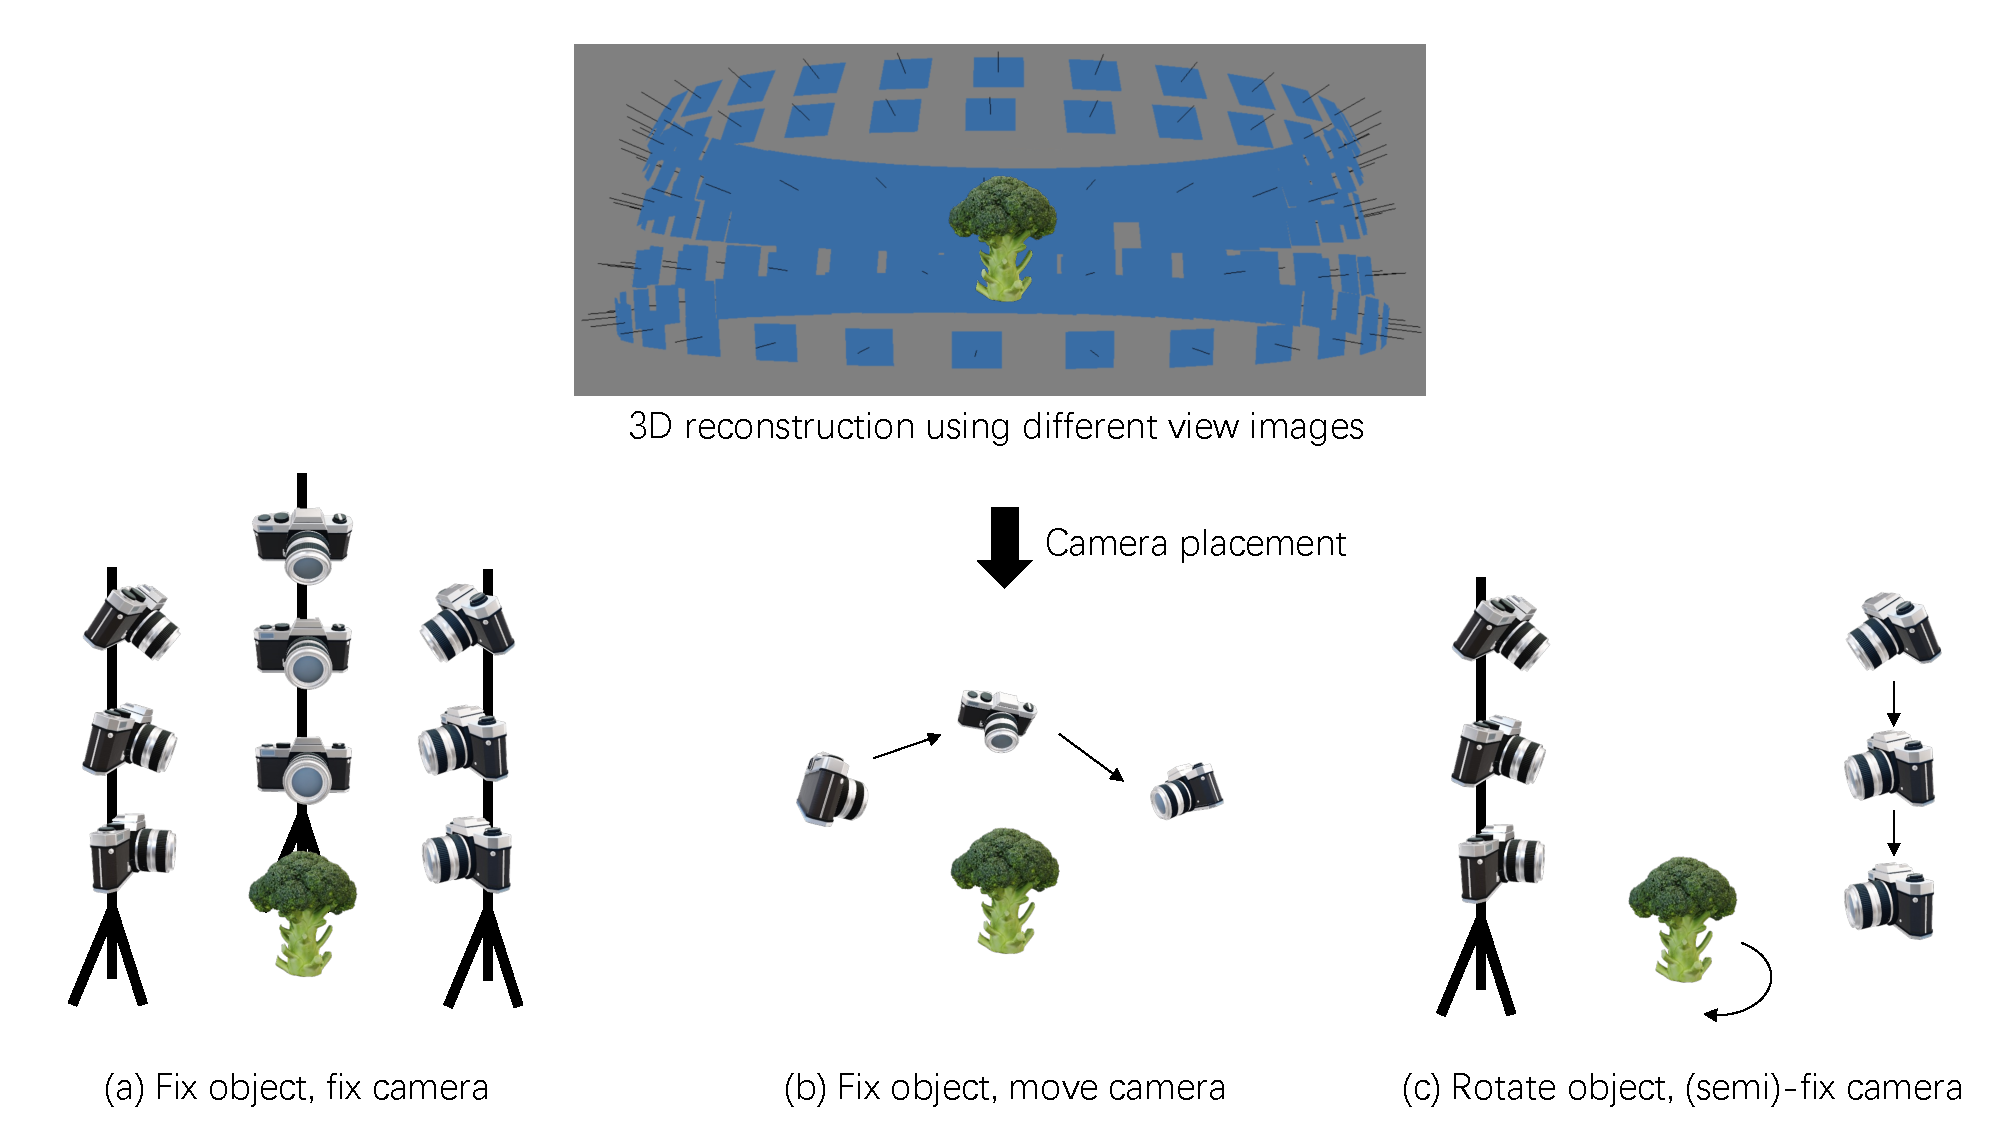
\includegraphics{figures/des/sfm_types.pdf}
    }
  \end{center}
  \caption[Current photogrammetry (3D reconstruction) methods and challenges]{
    The current photogrammetry (3D reconstruction) methods and challenges; (a-c) the current image acquisition approaches (a) fixing the object and taking images using multiple fixed cameras at the same time, also called forward intersection; (b) fixing the object but taking images by using a moved camera, also called backward resection; and (c) rotating the object and taking images using fewer multiple fixed cameras, or a camera fixed at different locations for each rotation. The challenges of current approaches: (d) the limited view angles of current image occlusion approaches has visual dead area, which will cause incomplete plant 3D models; and (e) the difficulties to segment foreground (plant) area in the image preprocessing.
  }
  \label{fig:des1}
\end{figure}

The first challenge is image acquisition for cost-effective reconstruction. Several authors used the following three approaches to acquire images (Fig.~\ref{fig:des1}): (a) fix the object and fix cameras \citep{nguyen_structured_2015}; (b) fix the object and move a camera manually \citep{xiao_image-based_2020} or using robotic arms \citep{cao_quantifying_2019,nguyen_3d_2016}; and (c) rotate the object and fix or move the camera(s) \citep{kochi_3d_2018,gao_novel_2021}. The main drawback of these imaging approaches is that it is difficult to provide fully complete perspectives of plants within acceptable cost. Most methods can only capture images of the sunlit side (such as the adaxial surface of leaves and the top of broccoli crowns); while capturing images of the shaded side (such as the abaxial surface of leaves and the downside of broccoli crowns) is more difficult and requires extreme upward viewing angles (Fig.~\ref{fig:des1}d). Even if such images can be acquired, they often fail to align with the 3D model due to insufficient feature matching points. Hence, a solution is required to improve the completion of the reconstructed plant 3D model, especially for solid, closed harvestable organs like broccoli heads.

The second challenge is image preprocessing for the acquired images. Compared to the approach of building the full scene, which includes both plants and backgrounds, following the segmenting of the plant parts \citep{ge_method_2019} and denoising \citep{wu_mvs-pheno_2020}; some studies segmented and masked the foreground (plant) area before doing the 3D reconstruction \citep{nguyen_3d_2016,kochi_3d_2018}, to improve the model quality and eliminate the effect of background noise. Although the controlled environment can provide pure background and stable lighting, it is still challenging to develop a robust algorithm to segment the broccoli area perfectly, especially to handle the shadows caused by the irregular broccoli head shape at the different growing stages. Some outdoor studies showed the power of deep learning for plant area detection and segmentation \citep{zhou_monitoring_2020,blok_effect_2021,garcia_towards_2021}, but due to limitation of the \gls{gpu} memory, the original images are often resized to smaller sizes for deep learning. For example, \citet{zhou_monitoring_2020} resized to $1440 \times 1080$, \citet{blok_effect_2021} resized to $1024 \times 1024$, and \citet{garcia_towards_2021} resized to $640 \times 480$. The plant mask produced in such a resolution can not fit well into the original images in detail (in our case, is $5184 \times 3456$), and hence also need a method to produce detailed masks with the original resolution.

In this study, several strategies were applied to overcome the previously mentioned challenges and provide a labor-saving pipeline for obtaining high-quality 3D models for destructively harvested broccoli heads. The objectives of this study were to (1) develop the dual-rotation object strategy with a fixed camera to collect images with abundant perspectives for complete 3D reconstruction; (2) implement the two-step deep learning workflow to acquire the detailed plant masks on the original images; (3) calculate the 3D morphological traits of broccoli head and crown; and (4) validate the estimated head size using the manual measurements. This pipeline also has great potential to be applied to other solid closed harvestable organs, such as oranges, potatoes, cauliflowers, and sweet potatoes, in which size is directly related to profit. Furthermore, using just a simple \gls{rgb} camera and several low-cost commercial photographic equipment, makes this pipeline more likely to be widely adopted.


\section{Methods and Materials}

The pipeline proposed in this study has two main parts, the workflow to acquire high-quality broccoli head 3D models and the workflow to measure the morphological traits of broccoli heads. For the first workflow, we developed an automatic imaging device using commercial photographic equipment, which extended the design of \citet{kochi_3d_2018} to dual-rotation of objects; then applied marker detection (software built-in function) and deep learning segmentation of plant masks to the collected images, as image preprocessing; afterward, we extended our previous batch scripts in \citet{feldman_easydcp_2021} to automatically operate the 3D reconstruction on a large number of broccoli heads to get 3D model results. For the second workflow, similar to our previous work \citep{feldman_easydcp_2021}, we first developed the unsupervised algorithm to split broccoli crown and stem parts; then corrected the broccoli head top direction of the 3D models (as the z-axis positive direction); lastly, we calculated several 2D and 3D morphological traits of the broccoli head and segmented crown.

\subsection{Plant materials}

Field trials were conducted at the experimental farm of the \gls{isas}, Nishi-Tokyo, Tokyo, Japan ($35^\circ 43'$N, $139^\circ 32'$E) from October 2021 to April 2022. The plot sizes were approximately $3000 m^2$; The meteorological data during the growth period were collected by a local weather station and are shown in Table~\ref{tbl:des1}. The soil was tilled and leveled using Half-Soiler and a Rotary implement. Initial fertilizer was mechanically spread and mixed thoroughly on October 11, 2021. From October 14 to 16 approximately 11,000 broccoli plants (cultivar: suzuka[すずか]) were machine transplanted with an in-row spacing of $35 cm$ and between-row spacing of $70 cm$. Additional fertilizer was applied by hand on October 28. Herbicides, insecticides, and fungicides were applied as needed using mechanical spreaders.

\begin{table}[htb]
  \caption{Meteorological data during the experiment period}
  \label{tbl:des1}
  % \begin{adjustwidth}{-0.05\textwidth}{-0.05\textwidth}
    \begin{center}
      \resizebox{1\textwidth}{!}{
        \begin{tabular}{cccc}
          \hline
                  & \begin{tabular}[c]{@{}c@{}}Mean temperature\\ ($^\circ C$)\end{tabular} & \begin{tabular}[c]{@{}c@{}}Total precipitation\\ ($mm$)\end{tabular} & \begin{tabular}[c]{@{}c@{}}Mean daily solar radiation\\ ($MJ \cdot m^{-2}$)\end{tabular} \\ \hline
          2021.10 & 17.6                                                                    & 156.5                                                                & 11.2                                                                                     \\
          2021.11 & 12.2                                                                    & 85.0                                                                 & 11.0                                                                                     \\
          2012.12 & 6.4                                                                     & 123.0                                                                & 9.6                                                                                      \\
          2022.01 & 3.6                                                                     & 16.5                                                                 & 10.6                                                                                     \\
          2022.02 & 3.8                                                                     & 60.0                                                                 & 13.3                                                                                     \\
          2022.03 & 10.3                                                                    & 94.5                                                                 & 15.3                                                                                     \\
          2022.04 & 15.0                                                                    & 213.0                                                                & 15.9                                                                                     \\ \hline
        \end{tabular}
      }
    \end{center}
  % \end{adjustwidth}
\end{table}

Three fertilizing treatments (inorganic, organic, and mixed) with three replicates (total 9 plots) were applied to produce different sizes and shapes of broccoli heads \citep{nishida_estimation_2023}. For each plot, several neighboured broccoli heads were destructively sampled during the flowering seasons (152 days after transplanting, Table~\ref{tbl:des2}) for indoor 3D reconstruction. 

\begin{table}[htb]
  \caption[Destructively sampled broccoli head number during the flowering season]{Destructively sampled broccoli head number during the flowering season. A total of 189 broccoli heads were destructively sampled. The ``rep'' means one replicate with 3 plots, while ``all'' means all 9 plots}
  \label{tbl:des2}
  % \begin{adjustwidth}{-0.05\textwidth}{-0.05\textwidth}
    \begin{center}
  %     \resizebox{1.1\textwidth}{!}{
          \begin{tabular}{cccc}
          \hline
          \textbf{Date} & \textbf{Plot id} & \textbf{head count} & \textbf{Total} \\ \hline
          Mar 17        & 3; 6; 9 (rep 3)  & 5 per plot          & 15             \\
          Mar 21        & 1; 4; 7 (rep 1)  & 5 per plot          & 15             \\
          Mar 24        & 2; 5; 8 (rep 2)  & 8 per plot          & 24             \\
          Mar 29        & 1-9 (all)        & 6 per plot          & 54             \\
          Mar 31        & 1-9 (all)        & 6 per plot          & 54             \\
          Apr 5         & 1-9 (all)        & 3 per plot          & 27             \\ \hline
          \end{tabular}
  %       \end{table}
  %     }
    \end{center}
  % \end{adjustwidth}
\end{table}

\subsection{Plant 3D model acquisition}

The general workflow to acquire a broccoli head 3D model is shown in Figure~\ref{fig:des_img_recons}, including imaging devices, image pre-processing, and batch reconstruction.

\begin{figure}[htb]
  \begin{center}
    \resizebox{\textwidth}{!}{
      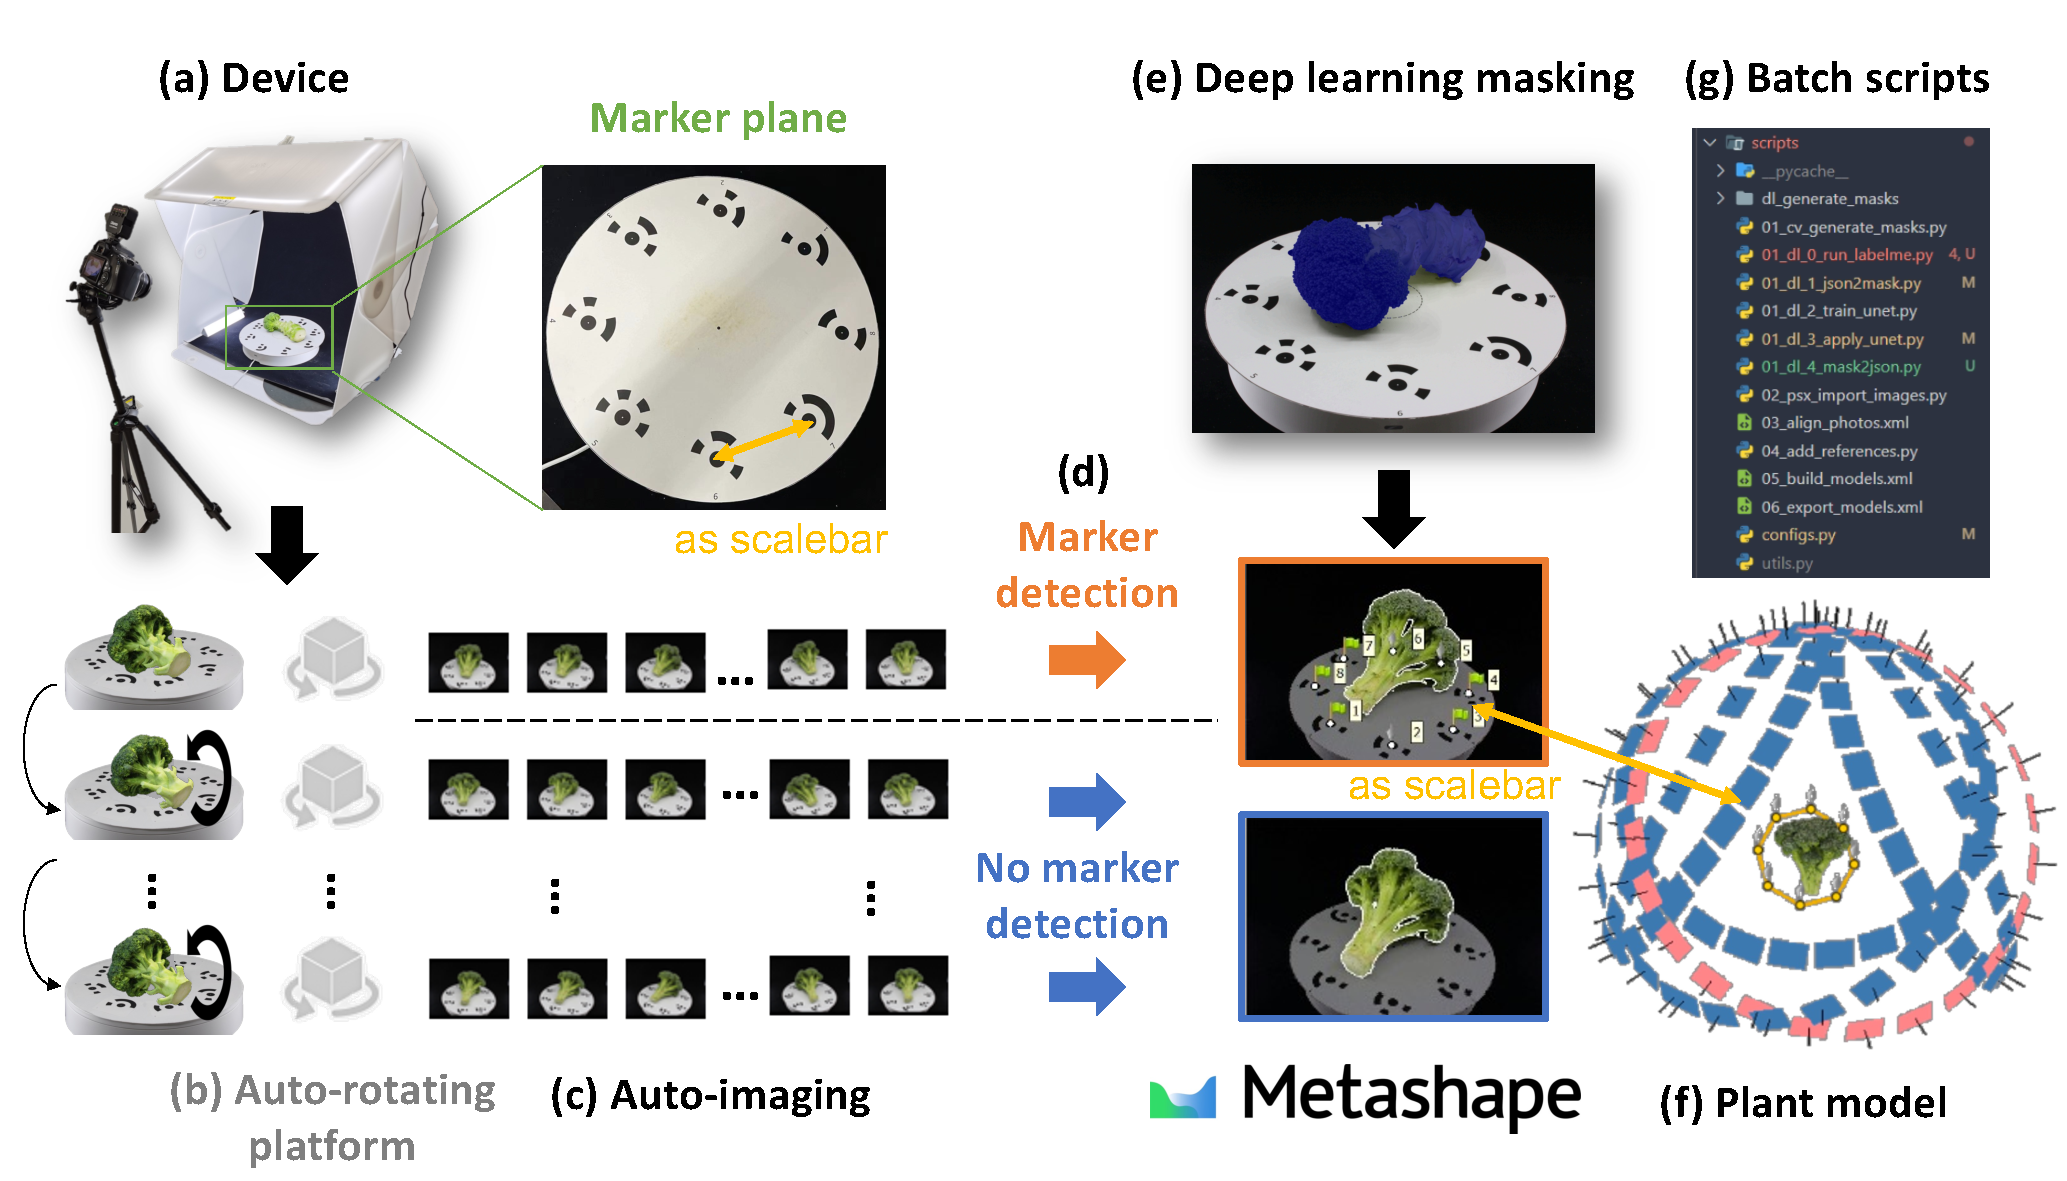
\includegraphics{figures/des/img_recons.pdf}
    }
  \end{center}
  \caption[The plant 3D model reconstruction workflow]{
    The Plant 3D model reconstruction workflow; (a) devices for taking plant images, with a marker plane used as scalebar references; (b) an automatic horizontal rotating platform, which can rotate at a given angle and then stop for a short interval for image taking. The vertical rotation of plants (flip) requires manual operation; (c) different photographic perspectives images taken by the infrared signal auto-imaging system; (d) partial marker detection to avoid misleading image alignment, where only markers on one rotating image group (orange) are detected and not on the others (blue); (e) plant part segmentation using deep learning; (f) the final 3D plant model produced by Metashape; and (g) the scripts for batch processing a large number of plants.
  }
  \label{fig:des_img_recons}
\end{figure}

The imaging device is assembled by a marker board, an automatic horizontal rotating platform (Foidio360, \url{https://orangemonkie.com/ja/products/foldio360-turntable}), a small photography studio (with lighting and pure color background), a Canon EOS 60D \gls{dslr} camera, and a tripod (Fig.~\ref{fig:des_img_recons}a). The rotating platform can rotate at a given angle ($15^\circ$ in this study) and then stop for a short interval for image taking. It was programmed to emit infrared signals to command the \gls{dslr} camera to take photos and then images were directly transferred to a computer through a data cable using Canon EOS Utility 2 software (\url{https://cweb.canon.jp/drv-upd/dc/euw21401.html}, Fig.~\ref{fig:des_img_recons}c). Manually rotating the broccoli head vertically (black rotation arrow in Fig.~\ref{fig:des_img_recons}b) to capture three to five photograph perspectives was required for complete 3D reconstruction. The commercial software, Agisoft Metashape (\url{https://www.agisoft.com}), was used for 3D reconstruction.

The 3D reconstruction and the later image and data processing were conducted on a computer with an AMD Ryzon 9 5950x with 16-Core processors, and DDR4 128GB \gls{ram}. The computer had one Nvidia GeForce RTX 3090 \gls{gpu}. The operating system is Windows 11 Professional. The codes are implemented in Python 3.8, \gls{cuda} 11.1, Pytorch 1.8.2, and torchversion 0.9.2.

The first step of image preprocessing is partial marker detection (Fig.~\ref{fig:des_img_recons}d). The marker board not only provides reference points for camera alignment but also provides the size calibration as a scalebar. The Agisoft Metashape 3D reconstruction software provides the built-in function to detect markers on the given images. However, only markers on the first rotating image group (orange color) are detected and not on the others (blue color). It was done since we vertically rotated the plants, thus changing the relationship between the plant and markers and potentially misleading the expected image alignment from other rotation groups. In other words, we want to ``cheat'' the software by inverting the relationship between static and rotating object. Thus, the software treats the broccoli as static and the camera as rotating (Fig.~\ref{fig:des_img_recons}f). The marker plane from the first image sequence was used for size calibration. Meanwhile, that marker plane was used as the X-Y plane for defining the 3D model coordinate.

Two pre-trained deep-learning networks were used for the second image processing step of plant area segmentation (masking). As mentioned in the introduction, deep learning can handle complicated image analyzing tasks, but often not with the original image resolution. Here we first use a pre-trained UNet with default model setting (\url{https://github.com/qubvel/segmentation_models.pytorch}) and do the transfer training with only 19 broccoli images. The training data is annotated using the open-source software, Labelme (\url{https://github.com/wkentaro/labelme}). The UNet model produces rough masks ($256 \times 256$ pixel resolution) with good performance and acceptable processing speed on almost all broccoli head images during the flowering season. Afterward, we directly use the pre-trained CascadePSP \citep[\url{https://github.com/hkchengrex/CascadePSP}]{cheng_cascadepsp_2020} to refine the rough masks to the original image resolution without any image annotation (Fig.~\ref{fig:des_img_recons}e). Afterward, to further address the potential flaws of the previous segmentation results, we assume the plant area should be one continuous region. Hence, only the largest region as the plant area was kept and the small holes inside the plant area was filled, as the final result.

Finally, the batch scripts were developed for the previous image preprocessing and the 3D reconstruction control in the Metashape (Fig.~\ref{fig:des_img_recons}g). The scripts and detailed use instructions can be found at \url{https://github.com/UTokyo-FieldPhenomics-Lab/Foldio360_3D_Reconstruct_Platform}.

\subsection{Morphological traits extraction}

The workflow of Morphological traits extraction is shown in Figure~\ref{fig:des_seg_alg}, which includes broccoli crown segmentation, direction correction, and trait calculation.

\begin{figure}[htbp!]
  \begin{center}
    \resizebox{0.9\textwidth}{!}{
      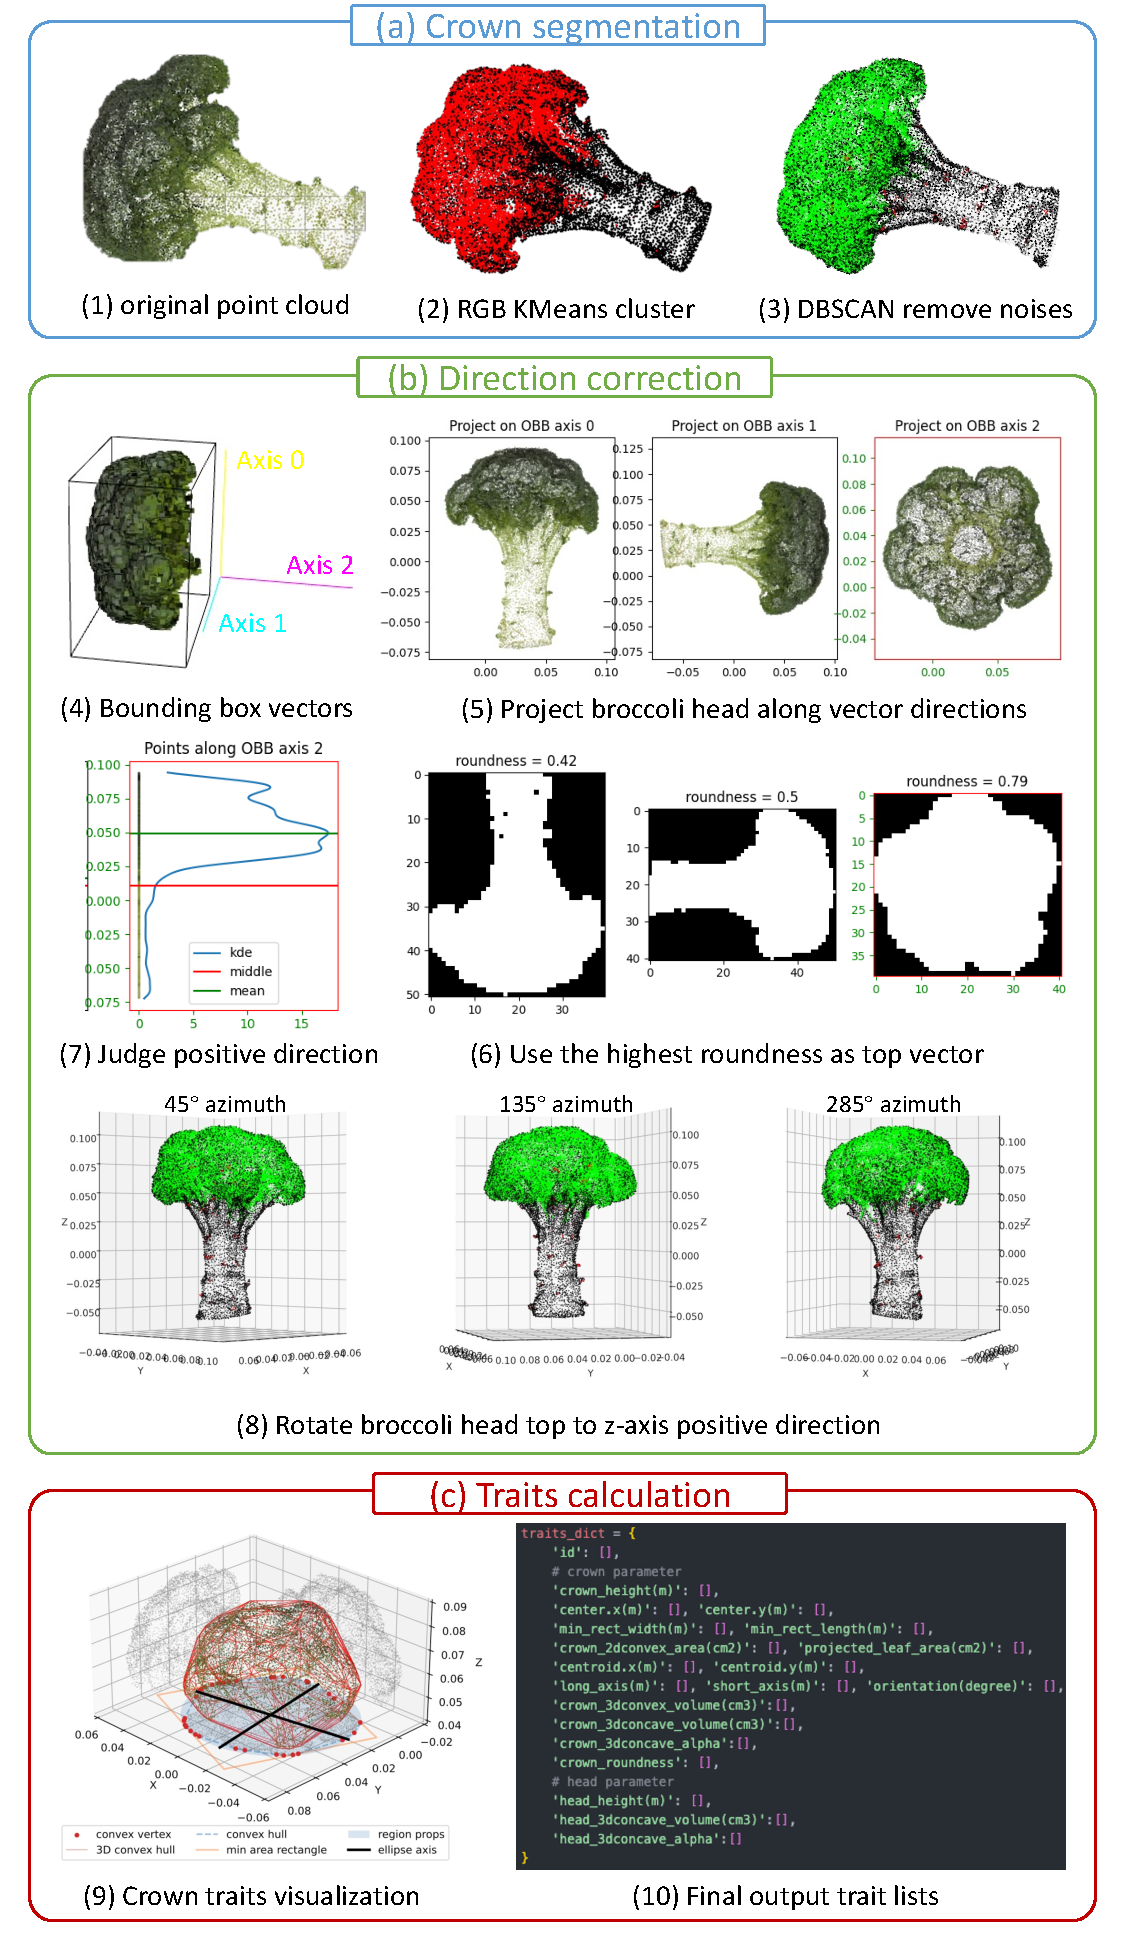
\includegraphics{figures/des/seg_algorithm.pdf}
    }
  \end{center}
  \caption[The algorithms for plant 3D model analysis]{
    The algorithms for plant 3D model analysis; (a) crown segmentation, to split the broccoli crown part and the stem part; (b) direction correction, to rotate the broccoli vertically to the z-axis positive direction; and (c) traits calculation.
  }
  \label{fig:des_seg_alg}
\end{figure}

The broccoli crown segmentation step aims to split the crown and the stem. Since they have significant color differences, the color information can be used for splitting. A method employed a simple color threshold, e.g. \citet{otsu_threshold_1979} did not work in a pilot study, because the color also varies among individual heads during the flowering season. Thus, a more robust method was developed. To begin, broccoli head 3D mesh models are transferred to a point cloud with \gls{rgb} colors (Fig.~\ref{fig:des_seg_alg}a1). An unsupervised Kmeans clustering algorithm splits all point clouds into two classes (Fig.~\ref{fig:des_seg_alg}a2). Later, the mean \gls{rgb} color values of these two classes are calculated and transformed into \gls{hsv} color space. The V represents the ``darkness'' of color, and the class with lower V values (darker color) is picked as the crown part. And finally, the \gls{dbscan} algorithm is used to cluster the crown points into several groups according to neighbor point density. These groups are clustered by 2-class Kmeans again according to their size, the clusters with smaller means sizes are discarded as noise (red dots in Fig.~\ref{fig:des_seg_alg}a3).

Due to the broccoli heads always laying on the marker board (the X-Y plane in the coordinates), the broccoli head top does not correspond to the z-axis positive direction for the reconstructed 3D model. Broccoli head top direction is corrected to better find the projecting plane for the crown projected area and crown thickness calculations. To begin, the minimum volume bounding box, also called \gls{obb}, and the vectors of its three perpendicular edges are calculated (Fig.~\ref{fig:des_seg_alg}b4). Since the broccoli head has variable shapes during the flowering season, the shortest perpendicular edge is not always the top direction. Hence, the full broccoli head is projected into the corresponding planes perpendicular to \gls{obb} vectors (Fig.~\ref{fig:des_seg_alg}b5); the roundness of the projected shape is also calculated. The vector with the highest roundness is used as the top direction vector (red boundary, Fig.~\ref{fig:des_seg_alg}b6). Later on, to find the positive direction (Axis 2 in Fig.~\ref{fig:des_seg_alg}b4 is a reversed direction), full broccoli along the vector (left greenish vertical line in Fig.~\ref{fig:des_seg_alg}b7) is projected; the middle value and the mean value of these points are also calculated. The positive direction should be the middle value greater than the mean value. The figure~\ref{fig:des_seg_alg}b8 shows the corrected direction along the previous vector, with azimuth angle views at $45^\circ$, $165^\circ$, and $285^\circ$.

In the end, similar to our previous work \citep{feldman_easydcp_2021}, we calculate the traits for the broccoli crown (Fig.~\ref{fig:des_seg_alg}c9) and the whole broccoli. For the 1D traits, we calculate the crown height (thickness) and whole broccoli height; For the 2D traits, we project the broccoli crown on the X-Y plane and calculate its center, centroid, roundness, minimum area rectangle width and length, projected area, convex hull area, and the short and long axis and azimuth angle of the fitted ellipse. For the 3D traits, we calculated the 3D convex hull volume for both the crown and whole broccoli and the 3D concave hull volume for the crown only (Fig.~\ref{fig:des_seg_alg}c10). 

The code for this section about broccoli head processing and traits calculating can be found at \url{https://github.com/UTokyo-FieldPhenomics-Lab/BroccoliHead3D.ipynb}

\subsection{Validation}

To further validate the workflow calculated traits with manually measured traits, and considering the difficulty of measuring 2D and 3D traits in reality, here we compared the size of broccoli head only. In agriculture practices, the head lengths are manually measured in the $0^\circ$, $45^\circ$, $90^\circ$, and $135^\circ$ directions (the ``union jack'' shape, \ding{107}) for validation. And then picking the longest and shortest ones as the final size. In the workflow calculated traits, the width and length of the minimum area rectangle, and the long and short axis of the fitted ellipse, have similar definitions as for head size descriptions. The agreement of workflow measured and manually measured is estimated using the coefficient of determination ($r^2$, calculated as the squared Pearson's correlation coefficient) and the \gls{rmse}:

\begin{equation}
  RMSE = \sqrt{\frac{1}{n} \cdot \sum_{i}^{n} (W_{i} - M_{i})^2}
\end{equation}

\noindent
where, $n$ is the total destructive sampled head number, $W_{i}$ is the \textbf{W}orkflow calculated length of broccoli head $i$, $M_{i}$ is the \textbf{M}anually measured length of broccoli head $i$.

\section{Results}

Following the workflow outlined above, a total of 189 destructively sampled broccoli heads were successfully 3D reconstructed during the flowering season with high model quality and completion. The intermediate results also show the feasibility of the proposed algorithms for variate broccoli head shapes. The calculated traits also have high correlations with manual measurements.

\subsection{Plant 3D model acquisition}

Figure~\ref{fig:des_dl_seg} shows some intermediate results for the plant area segmentation with variable broccoli head sizes and shapes. Using pre-trained UNet and transfer training with just 19 broccoli head images, rough masks (red parts in Fig.~\ref{fig:des_dl_seg}b) were successfully generated for different broccoli shapes. UNet image mask quality, especially on object boundaries, was limited by resolution and a low amount of training data. However, masks were substantially improved by CasadePSP and the hole-filling postprocessing (blue parts in Fig.~\ref{fig:des_dl_seg}c).

\begin{figure}[htb]
  \begin{center}
    \resizebox{\textwidth}{!}{
      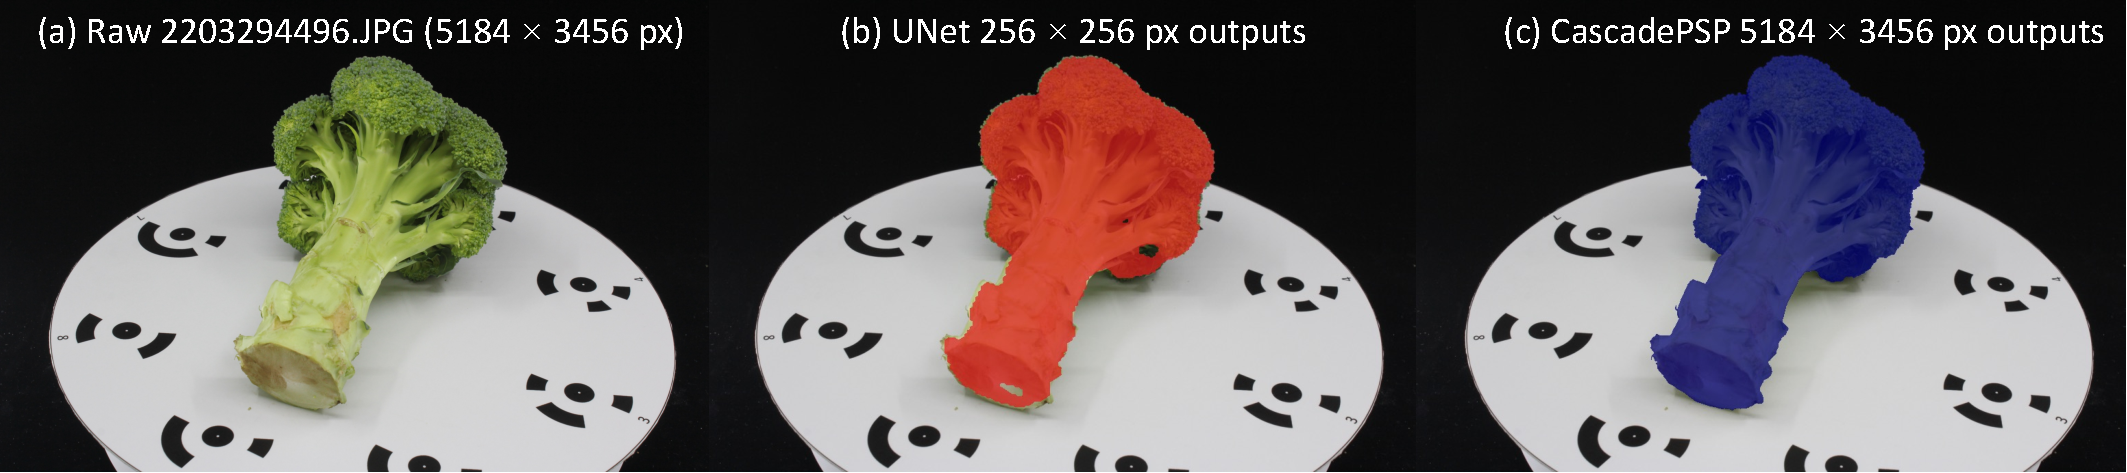
\includegraphics{figures/des/dl_seg.pdf}
    }
  \end{center}
  \caption[Two deep learning segmentation results]{
    An example of two deep learning segmentation results. (a) is the original image of broccoli head id ``2-11'' of rotating group 3, the resolution is $5184 \times 3456$ pixel; (b) is the output of the UNet segmentation, the resolution is $256 \times 256$ pixel, which is not enough as final plant masks; and (c) the output of the refined high-resolution mask using CasadePSP based on the UNet output. The mask has the same resolution as the original image.
  }
  \label{fig:des4}
\end{figure}

Some examples of reconstructed 3D head models are shown in Figure~\ref{fig:des_model_results}. Here we generate a \gls{cg} image using the 3D head models (Fig.~\ref{fig:des_model_results}b) and compare it visually to the real-world photo (Fig.~\ref{fig:des_model_results}a). Due to limitations in shooting angles and manual editing, the two images are not the same in detail, but the overall details and sizes of the broccoli are quite similar. Figure~\ref{fig:des_model_results}c shows different perspectives of the same broccoli head. Unlike other studies, in which the uderside of the model \citep{kochi_3d_2018} or leaf backside \citep{cao_quantifying_2019} are not available, the proposed pipeline does include the entire broccoli head, with bottoms of the crown and stem available. In general, our proposed dual-rotation workflow produces completely enclosed high-quality 3D models, it will not only contribute to better analysis accuracy but also build a base for future digital farm applications.

\begin{figure}[htb!]
  \begin{center}
    \resizebox{\textwidth}{!}{
      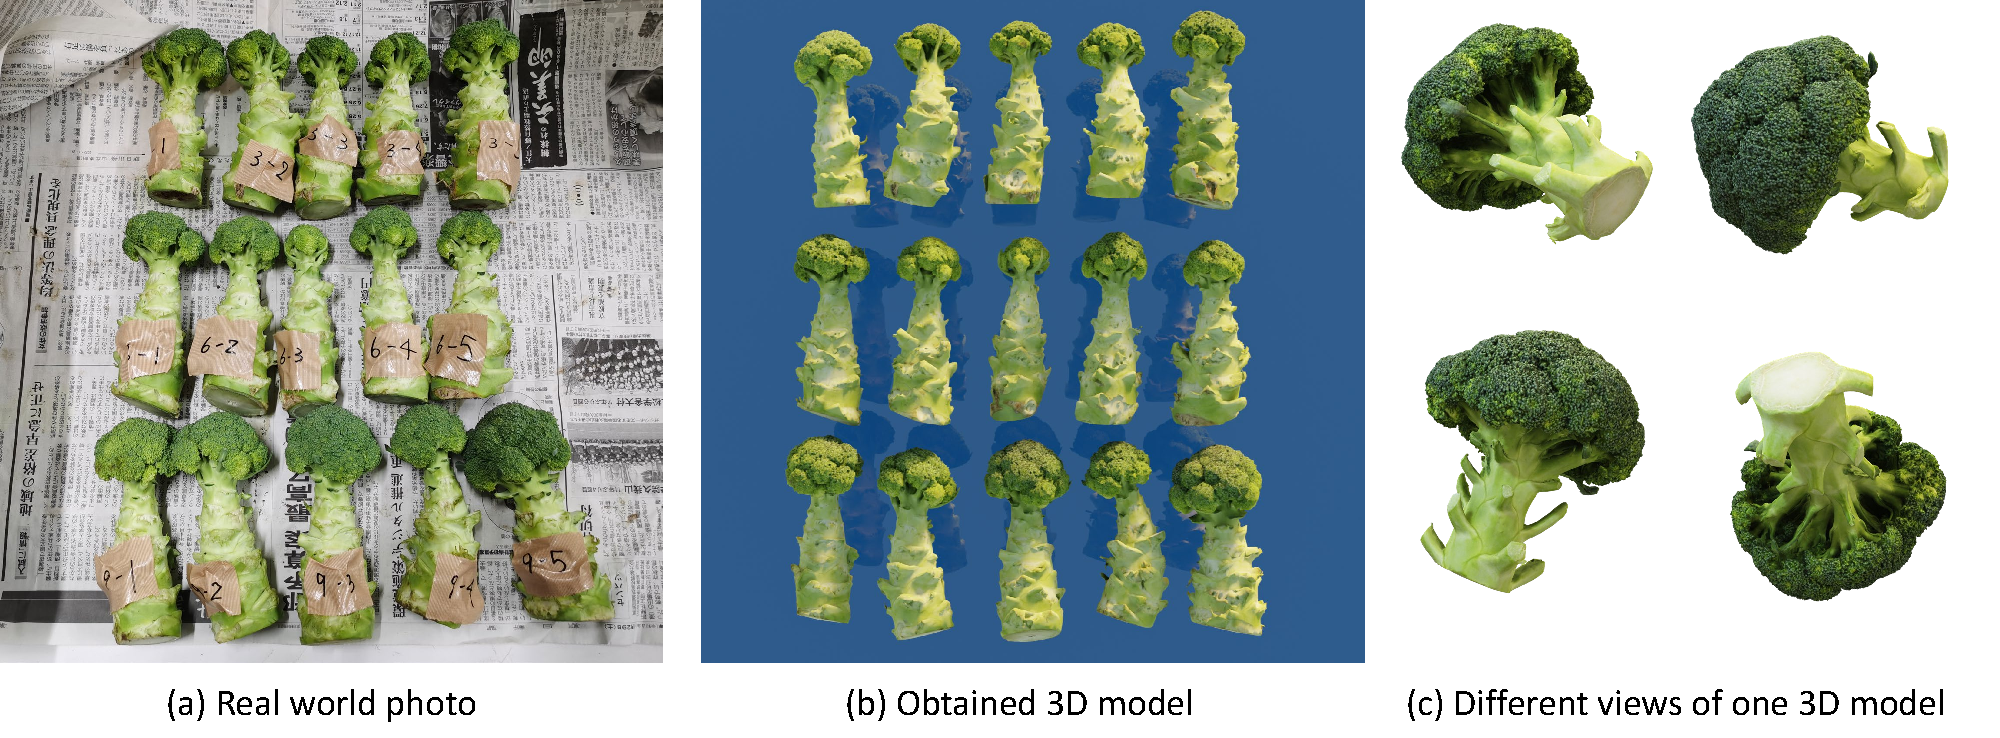
\includegraphics{figures/des/model_results.pdf}
    }
  \end{center}
  \caption[The obtained 3D models]{
    Some examples of obtained 3D models; (a) the image of 15 broccoli heads in the real world; (b) the obtained 3D models of corresponding broccoli heads; and (c) the different views of one broccoli head 3D model.
  }
  \label{fig:des_model_results}
\end{figure}

\subsection{Morphological traits extraction}

As mentioned before, the crown and stem parts of the broccoli head should be segmented and rotated upwards for easier trait calculation. Figure~\ref{fig:des_segrot} shows the feasibility of our proposed unsupervised algorithm on broccoli heads with different shapes. Figure~\ref{fig:des_segrot}a is a simple case of a small broccoli head with a straight stem; Figure~\ref{fig:des_segrot}b is a challenging case with a curved stem;  Figure~\ref{fig:des_segrot}c and d are challenging cases for head and stem segmentation. Instead of concluding that our algorithm rotates them to the exact status in the field correctly, it rotates them to a proper horizontal angle with the largest projection area on the X-Y plane and the shortest thickness on the Z-axis. This provides an initialized starting point for later trait calculation, especially very important for the 1D (on the Z-axis) traits and the 2D traits (on the X-Y plane).

\begin{figure*}[htb]
  \centering
  \begin{subfigure}[b]{0.475\textwidth}
    \centering
    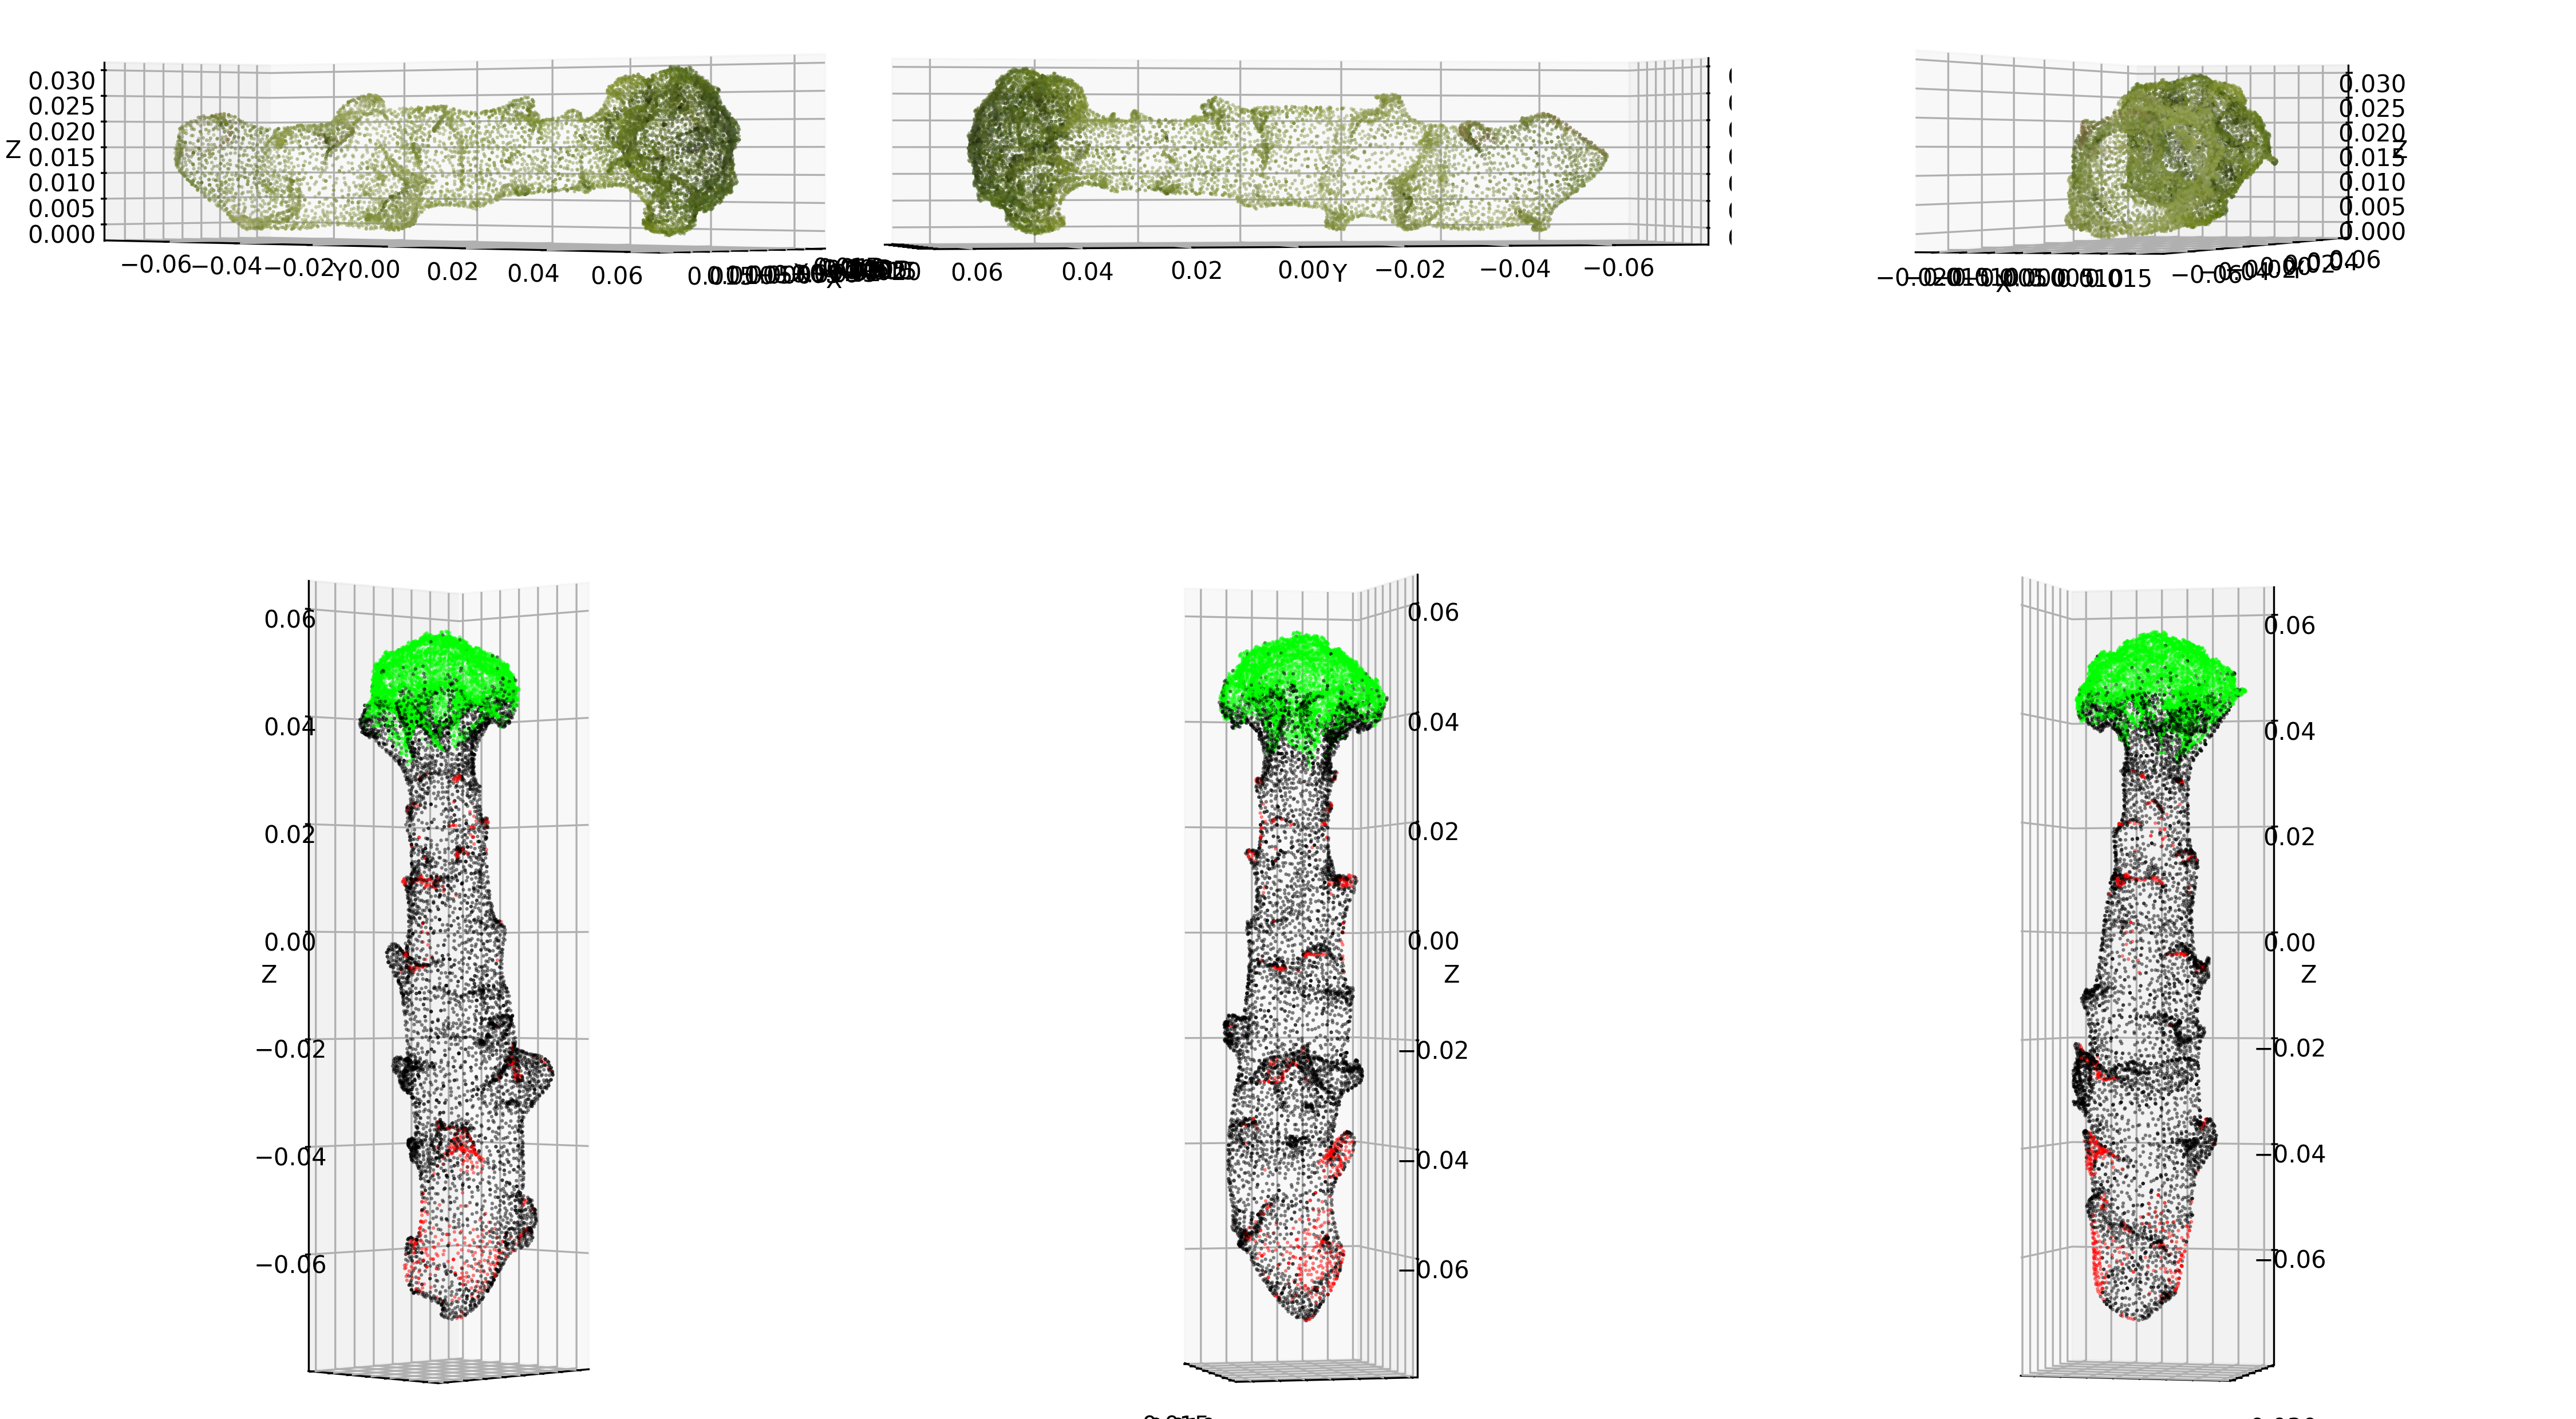
\includegraphics[width=\textwidth]{figures/des/7-2-2.png}
    \caption{ID 7-2-2}
  \end{subfigure}%
  \hfill
  \begin{subfigure}[b]{0.475\textwidth}
    \centering
    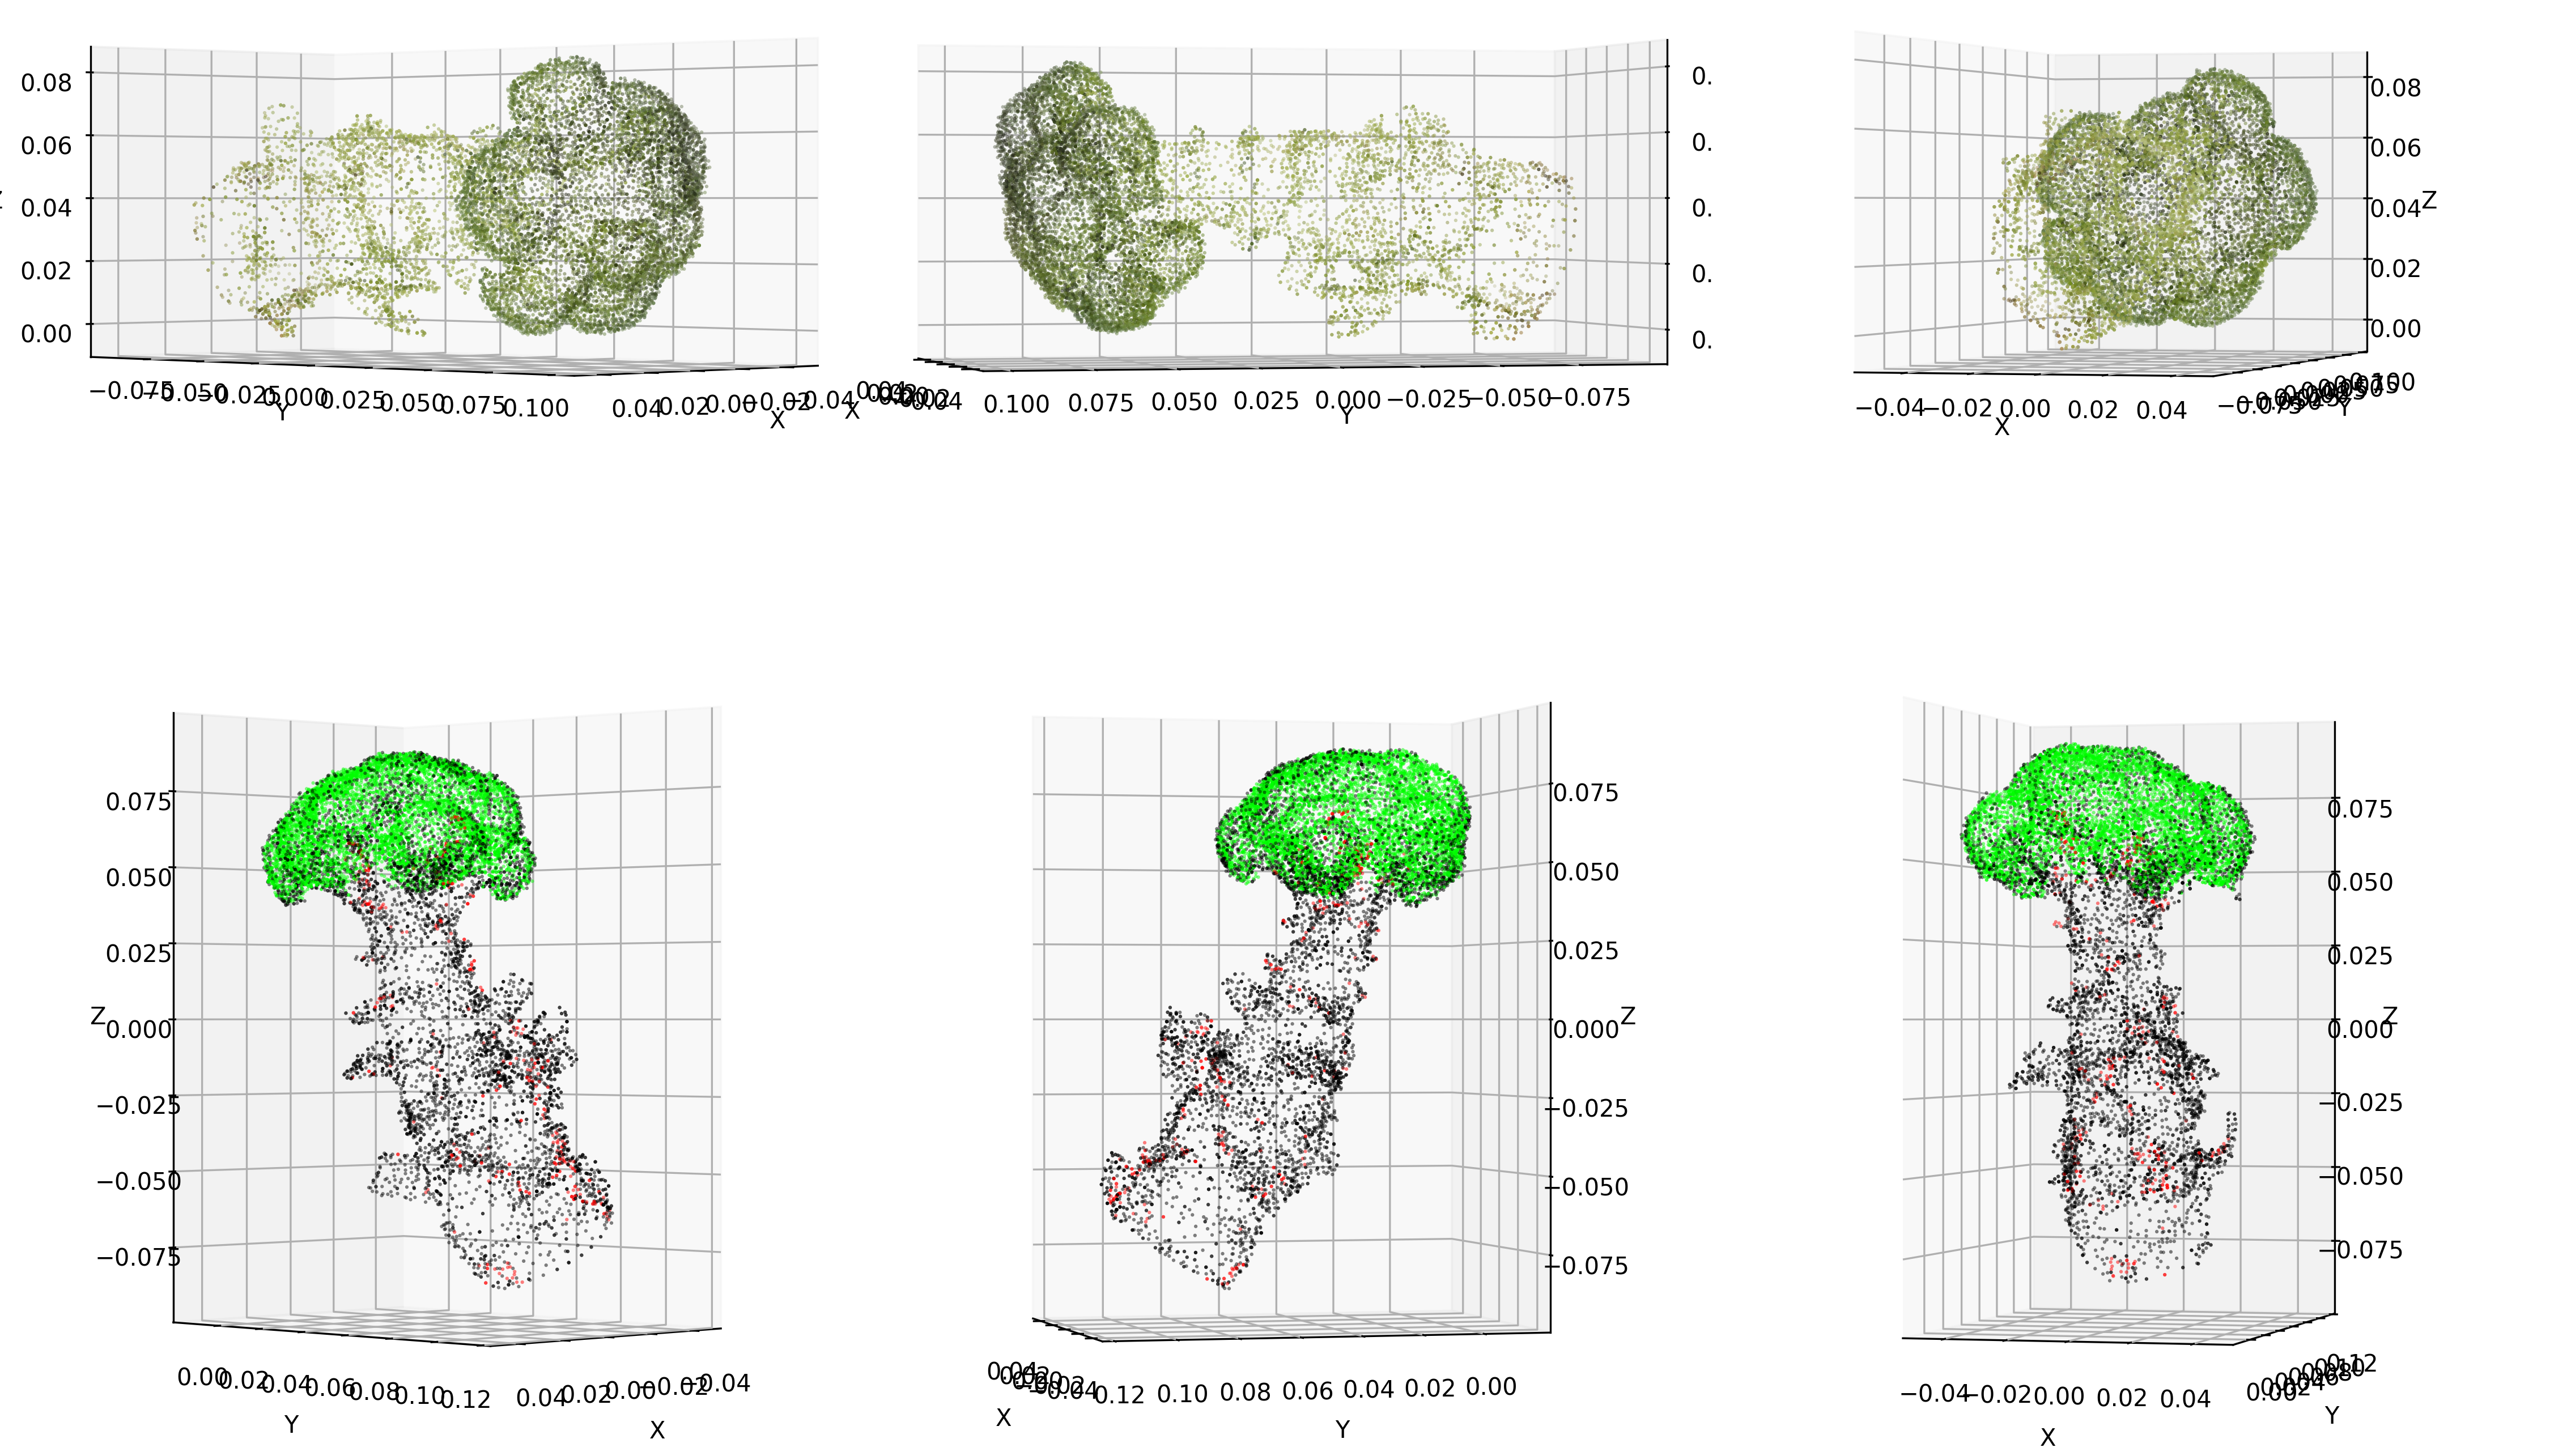
\includegraphics[width=\textwidth]{figures/des/1-5.png}
    \caption{ID 1-5}
  \end{subfigure}
  \vskip\baselineskip

  \begin{subfigure}[b]{0.475\textwidth}
    \centering
    \includegraphics[width=\textwidth]{figures/des/2-23.png}
    \caption{ID 2-23}
  \end{subfigure}%
  \hfill
  \begin{subfigure}[b]{0.475\textwidth}
    \centering
    \includegraphics[width=\textwidth]{figures/des/1-33.png}
    \caption{ID 1-33}
  \end{subfigure}%
  \caption[Examples of plant 3D model analysis at different growing stages]{
    Examples of plant 3D model analysis at different growing stages. The upper parts are the original coordinates of the obtained 3D models, while the lower parts are the segmented and direction-corrected results, the red parts are removed noises. Three columns show the corresponding azimuth angle views at $45^\circ$, $165^\circ$, and $285^\circ$ for the same 3D model.
  }
  \label{fig:des6}
\end{figure*}

To validate the accuracy of the proposed workflow calculated traits, they are compared with manual measurement using standard agricultural practices. Figure~\ref{fig:des_compare} shows the head size comparison results. The broccoli head size can be represented by the minimum area bounding rectangle and fitted ellipse axis lengths. Both the rectangle and the ellipse methods show high correlations with the manually measured results ($r^2\geq0.97$), but the rectangle has higher correlation than the ellipse. This is because the rectangle width and length are more like the minimum and maximum of the manually measured ``union jack (\ding{107})'' lengths, respectively. Assuming the complicated broccoli head is an ellipse inherently involves a certain degree of error, but the \gls{rmse}s of the ellipse assumption ($0.553 cm$ and $0.448 cm$) were still better than that of the circular assumption \citep[Table 5, \gls{rmse}$=0.97 cm$]{blok_image_2021}

\begin{figure}[htb!]
  \begin{center}
    \resizebox{\textwidth}{!}{
      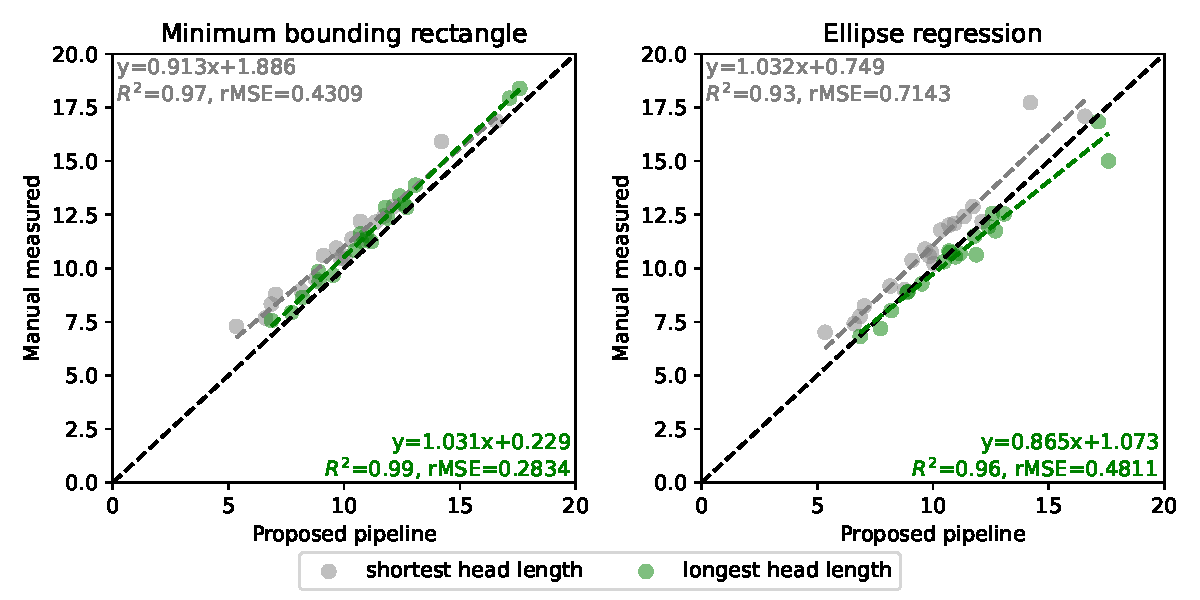
\includegraphics{figures/des/method_compare.pdf}
    }
  \end{center}
  \caption[The comparison between the proposed phenotyping pipeline and manual measurement]{
    The comparison between the proposed phenotyping pipeline and manual measurement. The shortest length and longest length of the broccoli head are compared. For the proposed pipeline, it uses two methods to estimate those lengths. One is using the length and width of the minimum bounding rectangle, the other is using the major and minor axes of the fitted ellipse.
  }
  \label{fig:des_compare}
\end{figure}

\section{Discussion}

In this study, we implement a 3D plant phenotyping pipeline to obtain high-quality 3D broccoli head models and calculate the 3D morphological traits of head shape and size. Our 3D model reconstruction method is superior to image acquisition methods used by many 3D-based phenotyping studies (Fig.~\ref{fig:des1}a-c), because they often fail to capture complete plant structure due to limited perspective. Here we extend the object rotation method (Fig.~\ref{fig:des1}c) to the dual-rotation (Fig.~\ref{fig:des_img_recons}d) using the commercial auto-rotation platform, which ensures enough perspectives without excessively increasing workload. Meanwhile, generating masks for the plant area on the images to exclude the impact of background noise has proved beneficial for 3D model quality. Rather than developing customized computer vision algorithms to extract plant area \citep{nguyen_3d_2016,kochi_3d_2018,kochi_all_2022}, which is not robust for different environments and plant objects, here we use the state-of-art pre-trained deep learning networks to decrease the workload of algorithm development and data annotation. The results show good feasibility of this pipeline on different shapes of broccoli heads during the flowering seasons. The open-source unsupervised algorithm to segment broccoli crown, correct the head direction and calculate several agronomically relevant traits is available here. 

Some questions or limitations remain; for example, the dual-rotation method is only suitable for solid objects, such as broccoli or cauliflower head or fruits. It cannot be applied to soft objects, such as flowers or plant leaves, whose shape or structure can change after vertical flipping on the marker plane. The object shape changing from different perspectives conflicts with the assumption of 3D reconstruction and results in poor model quality or even alignment failure. Secondly, the dual-rotation is also not fully automated, requiring manually flipping the object after each sequence of horizontally rotated images. Although flipping and replacing the broccoli only takes a few seconds each time, a person needs to be constantly waiting for each automation cycle to complete. The waiting time accounts for at least 80\% of the total imaging time. And lastly, limited by the developing time, we only publish the open-source code with simple instructions for this pipeline, there is no easy-to-use software with a friendly \gls{ui} for researchers without any programming background.

For future work, we plan to apply and examine the pipeline on more agricultural applications for crop organs, such as sweet potato quality judgment and potato tuber bud detection for agronimic, breeding and post-harvest quality objectives. The proposed pipeline also provides an ultra-high-quality broccoli head template database, which can integrate with the \gls{uav}-based outdoor survey for the full field to substantially improve model quality (In Chapter 3). Also, with the fast development of deep learning, more advanced models, like ``segment anything'' \citep{kirillov_segany_2023}, could be implemented to further reduce the workload in the image preprocessing process.

\section{Conclusion}

In this study, we have implemented an almost fully automated plant phenotyping pipeline based on the 3D reconstruction of broccoli heads. The described workflow has been designed to minimize the effects of limited perspective on the 3D model quality and completion. By using the dual-rotation of the object and the dual deep learning segmentation, our proposed workflow performed well on over 180 broccoli heads during the flowering season. The accuracy of pipeline calculated head size traits was validated by simple manual measurements using standard agricultural practices. The results suggest that our pipeline offers a great opportunity for high-throughput 3D phenotyping applications on the solid and enclosed plant organs (e.g. oranges, potatoes, cauliflowers, and sweet potatoes), in which size is directly related to harvest timing and profitability.